\chapter{Проектная часть}

\section{Описание моделей}

Для экспериментов были реализованы следующие модели:
\begin{itemize}
\item оконная (WindowNet) - данная модель подробно описана в разделе \ref{subsubsection:window},
\item сверточная (ConvNet) - данная модель подробно описана в разделе \ref{subsubsection:conv},
\item полносвязная нейронная сеть для работы с разреженными синтактико-семантическими признаками (ComprenoNet),
\item комбинация сверточной и полносвязной сети (ConvNet + ComprenoNet)
\end{itemize}

\subsection{Гиперпараметры моделей и признаки}

Общие для всех моделей гиперпараметры:
\begin{itemize}
\item $\alpha=0.01$ - шаг обучения,
\item $p=0.5$ - вероятность для Dropout слоя,
\item количество нейронов в последнем полносвязном слое равно 17,
т.к. используется схема IOBES. Четыре для каждого из четырех типов тегов и один для Outside.
\end{itemize}

Гиперпараметры для оконной модели (рис. \ref{figure:window_net}) следующие:
\begin{itemize}
\item $d_2 = 300$ - количество нейронов в полносвязном слое,
\item $K=5$ - величина окна. Если в окне нет слов, то окно дополняется специальным токеном PADDING,
\item $|T_s|=32$ - размер подмножества для пакетного градиентного спуска.
\end{itemize}

Гиперпараметры для сверточной модели (рис. \ref{figure:conv_net}) следующие:
\begin{itemize}
\item $d_2 = 300$ - количество нейронов в сверточном слое,
\item количество нейронов в полносвязном слое также равно 300,
\item $d_{win} = 3$ - величина окна. Если в окне нет слов, то окно дополняется специальным токеном PADDING,
\item $|T_s|=33$ - размер подмножества для пакетного градиентного спуска.
\end{itemize}

Для экспериментов были использованы следующие признаки:
\begin{itemize}
\item Embeddings - векторные представления слов Senna Embeddings,
\item Capitalization - дискретный признак капитализации слова с 5 возможными вариантами
(слово начинается с большой буквы, слово содержит большую букву,
все символы в слове состоят из больших букв, нет больших букв в слове, не слово),
\item Position - кодирование позиции слова в предложении (описано в разделе \ref{subsubsection:conv}),
\item Gazetteer - проверяется присутствие слова в газетире CoNLL 2003,
\item Compreno sparse features - синтактико-се\-ман\-ти\-ческие признаки Compreno размерности 83950,
\item Compreno SVD 1024 - синтактико-семантически признаки Compreno размерности 83950 были сжаты с использованием
модификации сингулярного разложения для работы с разреженными признаками
TruncatedSVD\footnote{http://scikit-learn.org/stable/modules/generated/sklearn.decomposition.TruncatedSVD.html}
до размерности 1024. После сжатия описываемая дисперсия была равна 72\%. Т.е. потерялось 28\% информации.
\end{itemize}

Все признаки, кроме Compreno sparse features, были включены в нейронные сети с использованием Lookup Table.


\subsection{ComprenoNet}

Архитектура и гиперпараметры полносвязной нейронной сети для работы с разреженными
синтактико-семантическими признаками (ComprenoNet) представлены ниже:
\begin{lstlisting}
input -> (1) -> (2) -> (3) -> (4) -> (5) -> (6) -> (7) -> output
(1): nn.SparseLinear(83951, 256)
(2): nn.Dropout(0.5)
(3): nn.HardTanh
(4): nn.Linear(256 -> 256)
(5): nn.Dropout(0.5)
(6): nn.HardTanh
(7): nn.Linear(256 -> 17)
\end{lstlisting}

SparseLinear представляет из себя обычный полносвязный слой (Linear), который
оптимизирован для работы с разреженными данными. Другие слои и процесс обучения
аналогичны тем, что были в разделе \ref{subsection:nn}.
Общий алгоритм работы сети следующий:
\begin{enumerate}
  \item На вход подается разреженный вектор признаков слова (размерность 83951) для которого предсказывается тег.
  \item Далее этот вектор пропускается через 2 полносвязных слоя.
  \item На выходе еще один полносвязный слой, который выдает вероятность определенного тега.
  Выходов также 17.
\end{enumerate}

\subsection{ConvNet + ComprenoNet}

Архитектура и гиперпараметры комбинации сверточной и полносвязной сети (ConvNet + ComprenoNet)
представлены на рис. \ref{figure:two_net}.
\begin{figure}[!h]
  \centering
  \caption{Комбинация сверточной и полносвязной сети (ConvNet + ComprenoNet)}
  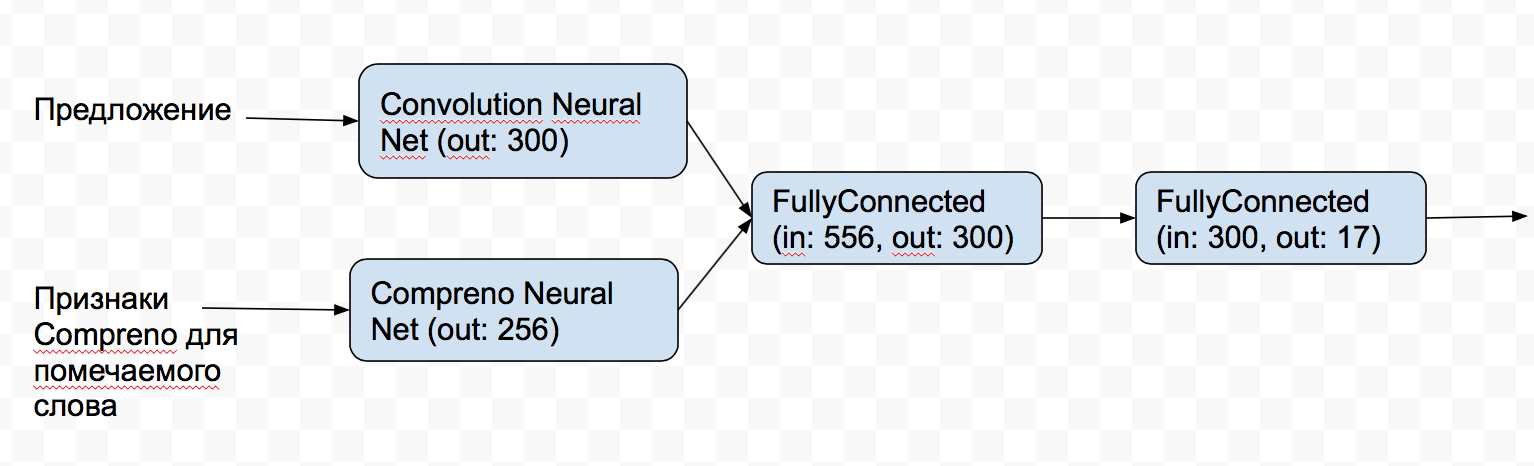
\includegraphics[scale=0.5]{figures/two-net.png}
  \label{figure:two_net}
\end{figure}
Эти сети соединяются следующим образом:
\begin{enumerate}
  \item Из обеих нейросетей удаляются выходные слои.
  \item Предыдущие слои из обеих сетей соединяются в новый полносвязный слой.
  \item Новый полносвязный слой соединяется с выходным слоем. Выходов как и тегов 17.
\end{enumerate}
Веса у объединенной сети были инициализированы предобученными моделями (ConvNet, ComprenoNet).

\section{Программная часть}

\subsection{Выбор программного фреймворка}

\subsection{Реализованная модель}

Нейронная сеть написана с использованием открытого фреймворка torch\footnote{http://torch.ch}.

Код для воспроизведения экспериментов выложен по адресу:
\href{https://github.com/sld/torch-conv-ner}{github.com/sld/torch-conv-ner}.

Скорость обучения на машине с GPU Amazon AWS g2.2xlarge\footnote{https://aws.amazon.com/ru/ec2/instance-types/}:
\begin{itemize}
\item 1 эпоха при одиночной обработке (stochastic gradient descent): $\sim$450 сек.
\item 1 эпоха при пакетной обработке (mini-batch gradient descent): $\sim$171 сек.
\item Модель получающая 87.49\% обучалась 91 эпоху ($\sim$4.2 часа).
\item 1 эпоха при пакетной обработке с использованием признаков Compreno: $\sim$615 сек.
\end{itemize}

Скорость классификации составляет 2500 токенов в секунду при пакетной обработке.
